\chapter{Sucursales}
\label{mod:15-sucursales}

\section{Propósito}
\label{sec:sucursales-proposito}

Vuelve a SIGA un sistema \textbf{multi-sucursal}: casi todo lo transaccional (stock, ventas, caja, timbrado, compras/recepciones, egresos, turnos/agenda, consultas clínicas) queda scopeado por sucursal, con transferencias de stock entre sucursales con flujo de aprobación. Es un proyecto transversal que tocó prácticamente todos los demás módulos del sistema, no solo las entidades propias listadas abajo.

\section{Entidades principales}
\label{sec:sucursales-entidades}

\begin{longtable}{p{3.6cm}p{9.6cm}}
\caption{Entidades principales del módulo de Sucursales.}
\label{tab:sucursales-entidades}\\
\toprule
\textbf{Entidad} & \textbf{Rol} \\
\midrule
\endfirsthead
\toprule
\textbf{Entidad} & \textbf{Rol} \\
\midrule
\endhead
\bottomrule
\endfoot
\code{Sucursal} & Unidad de scoping --- nombre, código único, ubicación (\code{Ciudad}). \\
\code{Transferencia}\allowbreak \code{Stock} & Cabecera de una transferencia entre dos sucursales (origen, destino, estado). \\
\code{Transferencia}\allowbreak \code{Stock}\allowbreak \code{Item} & Líneas de la transferencia (producto, cantidad). \\
\code{Ciudad} / \code{Departamento} & Catálogo de ubicación geográfica de Paraguay, reutilizado por \code{Sucursal} y \code{Proveedor}. \\
\end{longtable}

Además, \code{SucursalId} (FK) fue agregado a $\sim$15 entidades transaccionales ya documentadas en el capítulo de Modelo de Datos (Grupos A, B y C): \code{User}, \code{Horario}\allowbreak \code{Profesional}, \code{ConsultaClinica}, \code{Turno}, \code{MovimientoStock}, \code{StockLote}, \code{ConteoInventario}, \code{Venta}, \code{Timbrado}, \code{PedidoProveedor}, \code{Recepcion}\allowbreak \code{Mercaderia}, \code{Egreso} (y sus subtipos vía TPH), \code{SesionCaja}, \code{MovimientoCaja}. Quedan explícitamente \textbf{globales} (sin \code{SucursalId}): catálogos (\code{Producto}, \code{Marca}, \code{Servicio}, etc.) y personas (\code{Patient}, \code{Cliente}, \code{Professional}, y el \code{User} del admin).

\section{Reglas de negocio clave}
\label{sec:sucursales-reglas}

\begin{itemize}
  \item \textbf{Una sucursal fija por usuario, sin selector} --- ver \hyperref[adr:0009]{ADR 0009}. \code{User.SucursalId = null} significa usuario global (admin, y todos los pacientes por diseño). El scoping se resuelve centralmente en \code{ICurrent}\allowbreak \code{User}\allowbreak \code{Context} (\code{UserId}/\code{SucursalId}/\code{EsGlobal}/\code{TienePermiso}), no repetido en cada servicio.
  \item \textbf{La sucursal del staff se asigna desde el form de Profesional o de Empleado}, no desde la pantalla de Usuarios (esa solo gestiona roles + activar/desactivar).
  \item \textbf{Pacientes son globales}: no pertenecen a una sucursal fija, la eligen al reservar cada turno (paso propio en el modal de reserva).
  \item \textbf{\code{Producto}\allowbreak \code{Stock}\allowbreak \code{Config} (mín/máx de stock) quedó global por producto}, no por sucursal --- desvío de diseño explícito para no invalidar la relación 1:1 durante la migración.
  \item \textbf{\code{TrabajoPedido} no tiene \code{SucursalId} propio} --- deriva de \code{Venta.SucursalId} (el \code{Laboratorio}\allowbreak \code{Service} scopea a través de esa relación).
  \item \textbf{Transferencias de stock con flujo de aprobación}: crear = \code{Salida} en origen (estado \code{Pendiente}); aceptar = \code{Entrada} en destino; rechazar = \code{Entrada} de vuelta al origen. \textbf{Solo la sucursal destino gestiona} la aceptación o el rechazo --- la sucursal origen no puede cancelar unilateralmente una vez creada.
  \item \textbf{Usuario global (admin) ve y filtra todas las sucursales}; el resto del staff solo ve/opera la propia.
  \item \textbf{El scoping por sucursal de las $\sim$15 entidades listadas arriba sigue el mismo patrón centralizado en \code{ICurrent}\allowbreak \code{User}\allowbreak \code{Context}} descrito en el Capítulo~\ref{sec:arch}, \S\ref{sec:arch-multisucursal}.
\end{itemize}

\section{Endpoints}
\label{sec:sucursales-endpoints}

\begin{longtable}{p{2.6cm}p{5.4cm}p{5.2cm}}
\caption{Endpoints de Sucursales y Transferencias.}
\label{tab:sucursales-endpoints}\\
\toprule
\textbf{Método} & \textbf{Ruta} & \textbf{Descripción} \\
\midrule
\endfirsthead
\toprule
\textbf{Método} & \textbf{Ruta} & \textbf{Descripción} \\
\midrule
\endhead
\bottomrule
\endfoot
GET & \code{/}\allowbreak \code{api/}\allowbreak \code{sucursales?soloActivas} & Listado --- abierto a cualquier autenticado (incl.\ pacientes, lo necesitan para reservar turno) \\
GET & \code{/}\allowbreak \code{api/}\allowbreak \code{sucursales/}\allowbreak \code{{id}} & Detalle \\
POST / PUT / DELETE & \code{/}\allowbreak \code{api/}\allowbreak \code{sucursales(/}\allowbreak \code{{id})} & ABM, policy \code{gestionar_}\allowbreak \code{sucursales} \\
GET & \code{/}\allowbreak \code{api/}\allowbreak \code{transferencias?estado} & Listado, policy \code{transferir_stock} \\
POST & \code{/}\allowbreak \code{api/}\allowbreak \code{transferencias} & Crear (Salida en origen, \code{Pendiente}), policy \code{transferir_stock} \\
POST & \code{/}\allowbreak \code{api/}\allowbreak \code{transferencias/}\allowbreak \code{{id}/gestionar} & Aceptar/rechazar, policy \code{transferir_stock} \\
\end{longtable}

\section{Flujo típico}
\label{sec:sucursales-flujo}

Transferencia de stock entre dos sucursales (Figura~\ref{fig:seq-sucursales-transferencia}).

\begin{figure}[htbp]
\centering
% Nombres de actor en dos lineas y node distance corto: con los nombres
% completos en una linea la figura mide ~30cm y la mitad queda fuera de la
% pagina. Las notas al pie de la figura van centradas bajo el diagrama, no
% desplazadas a la derecha, por el mismo motivo.
\begin{tikzpicture}[node distance=0.7cm,
                    actor/.append style={font=\scriptsize\bfseries, minimum width=2.2cm}]
  \node[actor] (o) {Origen\\(staff)};
  \node[actor, right=of o] (api) {Transferencias\\Controller};
  \node[actor, right=of api] (svc) {TransferenciaStock\\Service};
  \node[actor, right=of svc] (s) {Movimiento\\Stock};
  \node[actor, right=of s] (d) {Destino\\(staff)};

  \draw[lineavida] (o.south) -- ++(0,-7.6);
  \draw[lineavida] (api.south) -- ++(0,-7.6);
  \draw[lineavida] (svc.south) -- ++(0,-7.6);
  \draw[lineavida] (s.south) -- ++(0,-7.6);
  \draw[lineavida] (d.south) -- ++(0,-7.6);

  \draw[mensaje] ($(o.south)+(0,-0.9)$) -- node[above,font=\scriptsize,align=center]{POST /transferencias\\(productos + destino)} ($(api.south)+(0,-0.9)$);
  \draw[mensaje] ($(api.south)+(0,-2.2)$) -- node[above,font=\scriptsize]{CreateAsync} ($(svc.south)+(0,-2.2)$);
  \draw[mensaje] ($(svc.south)+(0,-3.4)$) -- node[above,font=\scriptsize,align=center]{crear Salida en origen\\(valida stock)} ($(s.south)+(0,-3.4)$);
  \node[font=\tiny\itshape, align=center] at ($(svc.south)+(0,-4.4)$) {notifica a la sucursal destino (``transferencia pendiente'')\\TransferenciaStock queda en Estado = Pendiente};
  \draw[mensaje] ($(d.south)+(0,-5.8)$) -- node[above,font=\scriptsize,align=center]{POST /transferencias/\{id\}/gestionar\\(aceptar o rechazar)} ($(api.south)+(0,-5.8)$);
  \draw[mensaje] ($(svc.south)+(0,-7.0)$) -- node[above,font=\scriptsize,align=center]{aceptar: Entrada en destino\\rechazar: Entrada de vuelta en origen} ($(s.south)+(0,-7.0)$);
  \node[font=\tiny\itshape, align=center] at ($(svc.south)+(0,-8.2)$) {aceptar $\to$ Estado = Aceptada \quad rechazar $\to$ Estado = Rechazada};
\end{tikzpicture}
\caption{Transferencia de stock: crea Salida en origen (Pendiente); solo el destino gestiona la aceptación/rechazo.}
\label{fig:seq-sucursales-transferencia}
\end{figure}

\section{Vistas de frontend}
\label{sec:sucursales-frontend}

\begin{itemize}
  \item \code{SucursalesView.}\allowbreak \code{vue} --- ABM de sucursales (\code{/admin/sucursales}).
  \item \code{TransferenciasView.}\allowbreak \code{vue} --- crear transferencia (búsqueda de productos) + gestionar entrantes (aceptar/rechazar), ruta \code{/}\allowbreak \code{stock/}\allowbreak \code{transferencias}.
  \item Badge de sucursal en \code{AppHeader.vue} (componente, no vista): visible solo si el usuario tiene sucursal asignada (staff) o el permiso \code{ver_}\allowbreak \code{todas_}\allowbreak \code{sucursales} (admin $\to$ muestra ``Todas'').
  \item Paso de selección de sucursal en el modal de reserva de turno de \code{MisTurnosView.vue} (portal del paciente).
\end{itemize}

\section{Interfaz}
\label{sec:sucursales-interfaz}

\begin{figure}[htbp]
\centering
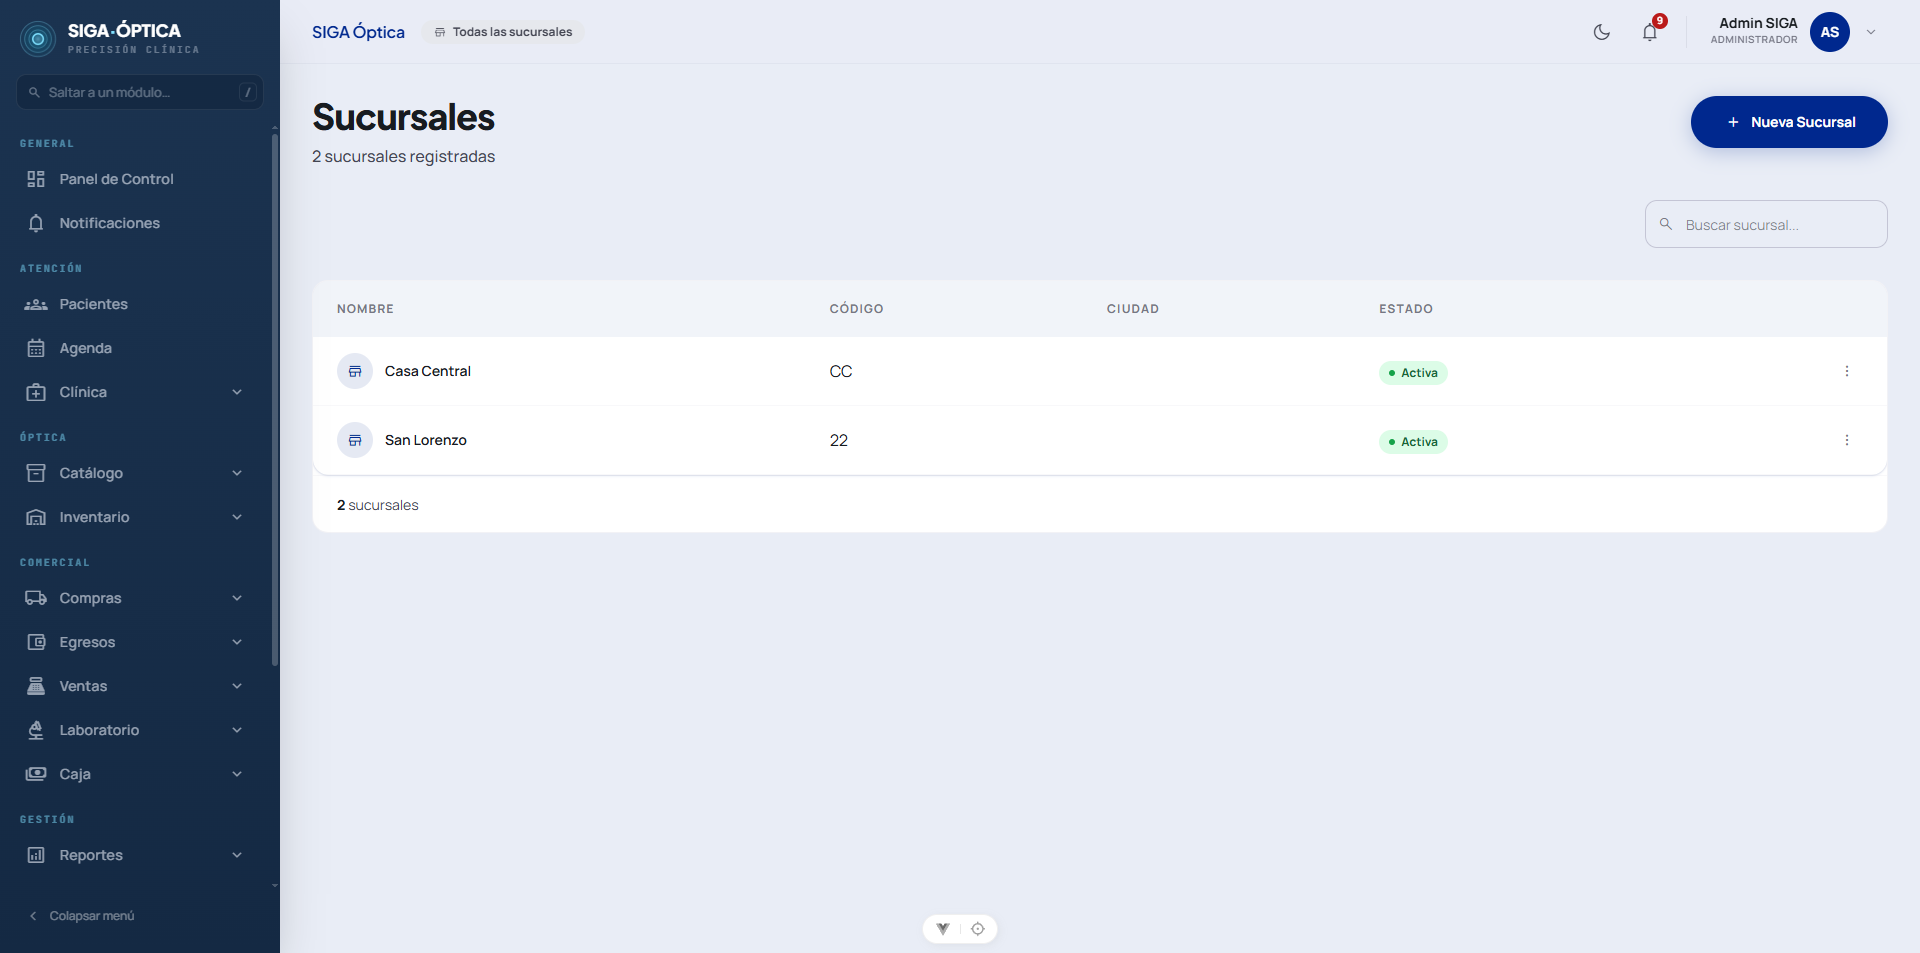
\includegraphics[width=0.95\textwidth]{imagenes/mod15-sucursales.png}
\caption{Listado de sucursales activas.}
\label{fig:mod15-sucursales}
\end{figure}

\section{Estado}
\label{sec:sucursales-estado}

\Implementado\ Las 7 fases del proyecto (0 a 6) están completas en código: Fase 0 (entidad Sucursal + CRUD + JWT + \code{ICurrent}\allowbreak \code{User}\allowbreak \code{Context} + permisos), Fase 1 (stock por sucursal), Fase 2 (ventas+caja+timbrado por sucursal), Fase 3 (compras+egresos por sucursal), Fase 4 (turnos/agenda+clínica por sucursal), Fase 5 (transferencias de stock), Fase 6 (reportes por sucursal). Migraciones \code{047} a \code{052}.
